% Options for packages loaded elsewhere
\PassOptionsToPackage{unicode}{hyperref}
\PassOptionsToPackage{hyphens}{url}
%
\documentclass[
  man,floatsintext]{apa6}
\usepackage{amsmath,amssymb}
\usepackage{iftex}
\ifPDFTeX
  \usepackage[T1]{fontenc}
  \usepackage[utf8]{inputenc}
  \usepackage{textcomp} % provide euro and other symbols
\else % if luatex or xetex
  \usepackage{unicode-math} % this also loads fontspec
  \defaultfontfeatures{Scale=MatchLowercase}
  \defaultfontfeatures[\rmfamily]{Ligatures=TeX,Scale=1}
\fi
\usepackage{lmodern}
\ifPDFTeX\else
  % xetex/luatex font selection
\fi
% Use upquote if available, for straight quotes in verbatim environments
\IfFileExists{upquote.sty}{\usepackage{upquote}}{}
\IfFileExists{microtype.sty}{% use microtype if available
  \usepackage[]{microtype}
  \UseMicrotypeSet[protrusion]{basicmath} % disable protrusion for tt fonts
}{}
\makeatletter
\@ifundefined{KOMAClassName}{% if non-KOMA class
  \IfFileExists{parskip.sty}{%
    \usepackage{parskip}
  }{% else
    \setlength{\parindent}{0pt}
    \setlength{\parskip}{6pt plus 2pt minus 1pt}}
}{% if KOMA class
  \KOMAoptions{parskip=half}}
\makeatother
\usepackage{xcolor}
\usepackage{longtable,booktabs,array}
\usepackage{calc} % for calculating minipage widths
% Correct order of tables after \paragraph or \subparagraph
\usepackage{etoolbox}
\makeatletter
\patchcmd\longtable{\par}{\if@noskipsec\mbox{}\fi\par}{}{}
\makeatother
% Allow footnotes in longtable head/foot
\IfFileExists{footnotehyper.sty}{\usepackage{footnotehyper}}{\usepackage{footnote}}
\makesavenoteenv{longtable}
\usepackage{graphicx}
\makeatletter
\newsavebox\pandoc@box
\newcommand*\pandocbounded[1]{% scales image to fit in text height/width
  \sbox\pandoc@box{#1}%
  \Gscale@div\@tempa{\textheight}{\dimexpr\ht\pandoc@box+\dp\pandoc@box\relax}%
  \Gscale@div\@tempb{\linewidth}{\wd\pandoc@box}%
  \ifdim\@tempb\p@<\@tempa\p@\let\@tempa\@tempb\fi% select the smaller of both
  \ifdim\@tempa\p@<\p@\scalebox{\@tempa}{\usebox\pandoc@box}%
  \else\usebox{\pandoc@box}%
  \fi%
}
% Set default figure placement to htbp
\def\fps@figure{htbp}
\makeatother
\setlength{\emergencystretch}{3em} % prevent overfull lines
\providecommand{\tightlist}{%
  \setlength{\itemsep}{0pt}\setlength{\parskip}{0pt}}
\setcounter{secnumdepth}{-\maxdimen} % remove section numbering
% Make \paragraph and \subparagraph free-standing
\makeatletter
\ifx\paragraph\undefined\else
  \let\oldparagraph\paragraph
  \renewcommand{\paragraph}{
    \@ifstar
      \xxxParagraphStar
      \xxxParagraphNoStar
  }
  \newcommand{\xxxParagraphStar}[1]{\oldparagraph*{#1}\mbox{}}
  \newcommand{\xxxParagraphNoStar}[1]{\oldparagraph{#1}\mbox{}}
\fi
\ifx\subparagraph\undefined\else
  \let\oldsubparagraph\subparagraph
  \renewcommand{\subparagraph}{
    \@ifstar
      \xxxSubParagraphStar
      \xxxSubParagraphNoStar
  }
  \newcommand{\xxxSubParagraphStar}[1]{\oldsubparagraph*{#1}\mbox{}}
  \newcommand{\xxxSubParagraphNoStar}[1]{\oldsubparagraph{#1}\mbox{}}
\fi
\makeatother
% definitions for citeproc citations
\NewDocumentCommand\citeproctext{}{}
\NewDocumentCommand\citeproc{mm}{%
  \begingroup\def\citeproctext{#2}\cite{#1}\endgroup}
\makeatletter
 % allow citations to break across lines
 \let\@cite@ofmt\@firstofone
 % avoid brackets around text for \cite:
 \def\@biblabel#1{}
 \def\@cite#1#2{{#1\if@tempswa , #2\fi}}
\makeatother
\newlength{\cslhangindent}
\setlength{\cslhangindent}{1.5em}
\newlength{\csllabelwidth}
\setlength{\csllabelwidth}{3em}
\newenvironment{CSLReferences}[2] % #1 hanging-indent, #2 entry-spacing
 {\begin{list}{}{%
  \setlength{\itemindent}{0pt}
  \setlength{\leftmargin}{0pt}
  \setlength{\parsep}{0pt}
  % turn on hanging indent if param 1 is 1
  \ifodd #1
   \setlength{\leftmargin}{\cslhangindent}
   \setlength{\itemindent}{-1\cslhangindent}
  \fi
  % set entry spacing
  \setlength{\itemsep}{#2\baselineskip}}}
 {\end{list}}
\usepackage{calc}
\newcommand{\CSLBlock}[1]{\hfill\break\parbox[t]{\linewidth}{\strut\ignorespaces#1\strut}}
\newcommand{\CSLLeftMargin}[1]{\parbox[t]{\csllabelwidth}{\strut#1\strut}}
\newcommand{\CSLRightInline}[1]{\parbox[t]{\linewidth - \csllabelwidth}{\strut#1\strut}}
\newcommand{\CSLIndent}[1]{\hspace{\cslhangindent}#1}
\ifLuaTeX
\usepackage[bidi=basic]{babel}
\else
\usepackage[bidi=default]{babel}
\fi
\babelprovide[main,import]{english}
% get rid of language-specific shorthands (see #6817):
\let\LanguageShortHands\languageshorthands
\def\languageshorthands#1{}
\ifLuaTeX
  \usepackage[english]{selnolig} % disable illegal ligatures
\fi
% Manuscript styling
\usepackage{upgreek}
\captionsetup{font=singlespacing,justification=justified}

% Table formatting
\usepackage{longtable}
\usepackage{lscape}
% \usepackage[counterclockwise]{rotating}   % Landscape page setup for large tables
\usepackage{multirow}		% Table styling
\usepackage{tabularx}		% Control Column width
\usepackage[flushleft]{threeparttable}	% Allows for three part tables with a specified notes section
\usepackage{threeparttablex}            % Lets threeparttable work with longtable

% Create new environments so endfloat can handle them
% \newenvironment{ltable}
%   {\begin{landscape}\centering\begin{threeparttable}}
%   {\end{threeparttable}\end{landscape}}
\newenvironment{lltable}{\begin{landscape}\centering\begin{ThreePartTable}}{\end{ThreePartTable}\end{landscape}}

% Enables adjusting longtable caption width to table width
% Solution found at http://golatex.de/longtable-mit-caption-so-breit-wie-die-tabelle-t15767.html
\makeatletter
\newcommand\LastLTentrywidth{1em}
\newlength\longtablewidth
\setlength{\longtablewidth}{1in}
\newcommand{\getlongtablewidth}{\begingroup \ifcsname LT@\roman{LT@tables}\endcsname \global\longtablewidth=0pt \renewcommand{\LT@entry}[2]{\global\advance\longtablewidth by ##2\relax\gdef\LastLTentrywidth{##2}}\@nameuse{LT@\roman{LT@tables}} \fi \endgroup}

% \setlength{\parindent}{0.5in}
% \setlength{\parskip}{0pt plus 0pt minus 0pt}

% Overwrite redefinition of paragraph and subparagraph by the default LaTeX template
% See https://github.com/crsh/papaja/issues/292
\makeatletter
\renewcommand{\paragraph}{\@startsection{paragraph}{4}{\parindent}%
  {0\baselineskip \@plus 0.2ex \@minus 0.2ex}%
  {-1em}%
  {\normalfont\normalsize\bfseries\itshape\typesectitle}}

\renewcommand{\subparagraph}[1]{\@startsection{subparagraph}{5}{1em}%
  {0\baselineskip \@plus 0.2ex \@minus 0.2ex}%
  {-\z@\relax}%
  {\normalfont\normalsize\itshape\hspace{\parindent}{#1}\textit{\addperi}}{\relax}}
\makeatother

\makeatletter
\usepackage{etoolbox}
\patchcmd{\maketitle}
  {\section{\normalfont\normalsize\abstractname}}
  {\section*{\normalfont\normalsize\abstractname}}
  {}{\typeout{Failed to patch abstract.}}
\patchcmd{\maketitle}
  {\section{\protect\normalfont{\@title}}}
  {\section*{\protect\normalfont{\@title}}}
  {}{\typeout{Failed to patch title.}}
\makeatother

\usepackage{xpatch}
\makeatletter
\xapptocmd\appendix
  {\xapptocmd\section
    {\addcontentsline{toc}{section}{\appendixname\ifoneappendix\else~\theappendix\fi: #1}}
    {}{\InnerPatchFailed}%
  }
{}{\PatchFailed}
\makeatother
\keywords{keywords\newline\indent Word count: X}
\usepackage{csquotes}
\usepackage{bookmark}
\IfFileExists{xurl.sty}{\usepackage{xurl}}{} % add URL line breaks if available
\urlstyle{same}
\hypersetup{
  pdftitle={The Interplay of Race/Ethnicity and Parental Education in College Completion: A Cohort Analysis},
  pdfauthor={Christopher Byrd1},
  pdflang={en-EN},
  pdfkeywords={keywords},
  hidelinks,
  pdfcreator={LaTeX via pandoc}}

\title{The Interplay of Race/Ethnicity and Parental Education in College Completion: A Cohort Analysis}
\author{Christopher Byrd\textsuperscript{1}}
\date{}


\shorttitle{The Interplay of Race/Ethnicity and Parental}

\authornote{

Whitworth University Sociology Department, Criminology Major. \url{https://orcid.org/0009-0004-0100-0798}

Correspondence concerning this article should be addressed to Christopher Byrd, 300 W Hawthorne Rd, Spokane, WA 99251. E-mail: \href{mailto:cbyrd25@my.whitworth.edu}{\nolinkurl{cbyrd25@my.whitworth.edu}}

}

\affiliation{\vspace{0.5cm}\textsuperscript{1} Whitworth University}

\abstract{%
One or two sentences providing a \textbf{basic introduction} to the field, comprehensible to a scientist in any discipline.
Two to three sentences of \textbf{more detailed background}, comprehensible to scientists in related disciplines.
One sentence clearly stating the \textbf{general problem} being addressed by this particular study.
One sentence summarizing the main result (with the words ``\textbf{here we show}'' or their equivalent).
Two or three sentences explaining what the \textbf{main result} reveals in direct comparison to what was thought to be the case previously, or how the main result adds to previous knowledge.
One or two sentences to put the results into a more \textbf{general context}.
Two or three sentences to provide a \textbf{broader perspective}, readily comprehensible to a scientist in any discipline.
}



\begin{document}
\maketitle

The United States features a diverse system of education. As diverse as the processes between states and districts is the students who reside in each, with further divisions manifesting themselves in differing educational outcomes.

Among U.S. adults born from 1980 to 1984, how does the intersection of race/ethnicity and parental education affect completion of a bachelor's degree or higher by 2017 (age's 33-37)? This question is of particular interest as educational inequality is rampant in the united states

\section{Literature Review (1.5-3 pg)}\label{literature-review-1.5-3-pg}

• What have others written about these subjects? • What theoretical approach are you interacting with? • Use the literature to make a case for why your project is necessary. State your hypothesis. This does not need to be in a separate section, put it where it fits in your paper. Be sure to describe your expectations and explain your logic. (.5-1 pg)

\section{Methods (1.5-2.5 pg)}\label{methods-1.5-2.5-pg}

As previously described, the sample used was the National Longitudinal Survey of Youth 1997 (NLSY97) conducted by the US Bureau of Labor Statistics (BLS). This is a nationally representative sample carried out every year pre-2011 and every two years thereafter, with selection finalized in 1997 and round 0 of questions carried out in 1998. This database was chosen due to it's large sample size (\textasciitilde8,000 respondents), robust and comprehensive question selection, representative nature, and ease of access. The sampling strategy, as described by the BLS, is as follows:

\begin{quote}
The NLSY97 cohort was selected in two phases\ldots{} In the first phase, a list of housing units for the cross-sectional sample and the over-sample was derived from two independently selected, stratified multistage area probability samples. This ensured an accurate representation of different sections of the population defined by race, income, region, and other factors. In the second phase, sub-samples of the eligible persons identified in the first phase were selected for interview.
\end{quote}

Additional information about the NLSY97 is available on the NLS website \href{https://www.nlsinfo.org/content/cohorts/nlsy97}{here}.

Within the NLSY97, the data was subset to specify participants in round 18 who responded with an answer to the following question: {[}What is{]} the highest degree received as of the survey date? This was on a scale of of 0 to 7, with zero representing no high school completion and 7 representing a doctorates degree. Important to note is the difference in scales between parental and respondent education levels (see appendix A for the complete codebook).

A unique aspect of the data which made analysis more complex was the number of answers missing from the residential dad educational variable (round 1). Residential dad was chosen, as this study is attempting to determine how parents living in the same household affect their children's future education. To determine whether the pattern was random, Jamshidian and Jalal's (2010) Non-Parametric MCAR Test. Following this, data was imputed using the mice package, which utilizes Gibbs sampling. The imputation method chosen was predictive mean matching (PMM), as PMM provides plausible data that is more robust than other methods (Buuren, 2018).

Following

• Identify population, describe sampling strategy and why you chose that strategy. • What are the indicators of your variables? • How did you actually carry out the research? (study design and process) • Describe your data analysis -- statistical test if quant or coding process if qual • Why is this context and this method the best choice for your research question?

\section{Results (1-2 pg)}\label{results-1-2-pg}

The

\begin{figure}
\centering
\pandocbounded{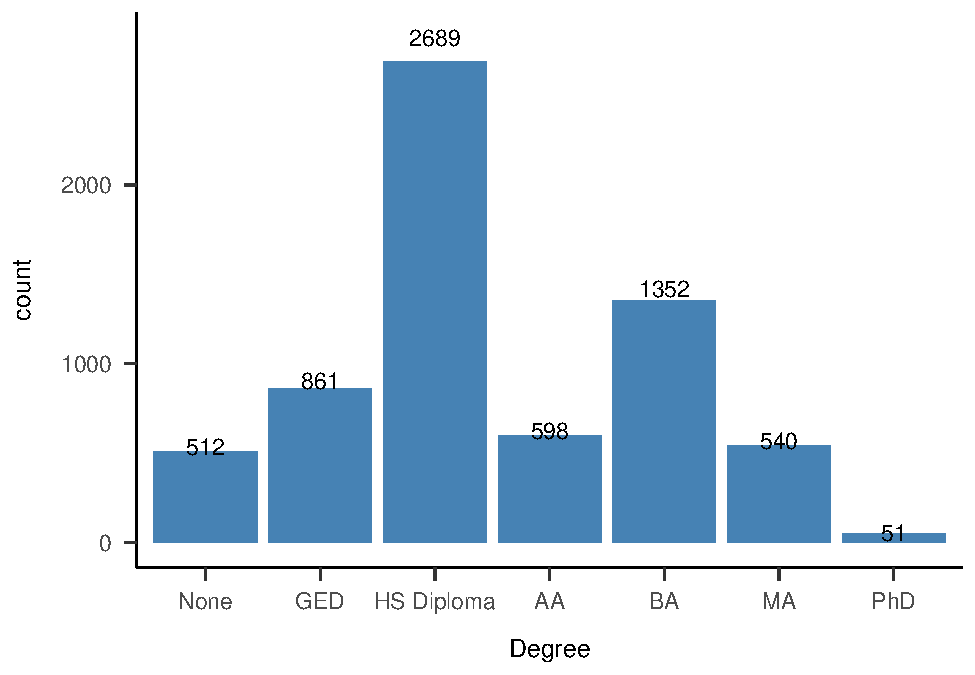
\includegraphics[keepaspectratio]{tables_files/figure-latex/unnamed-chunk-1-1.pdf}}
\caption{\label{fig:unnamed-chunk-1}Fig}
\end{figure}

\begin{figure}
\centering
\pandocbounded{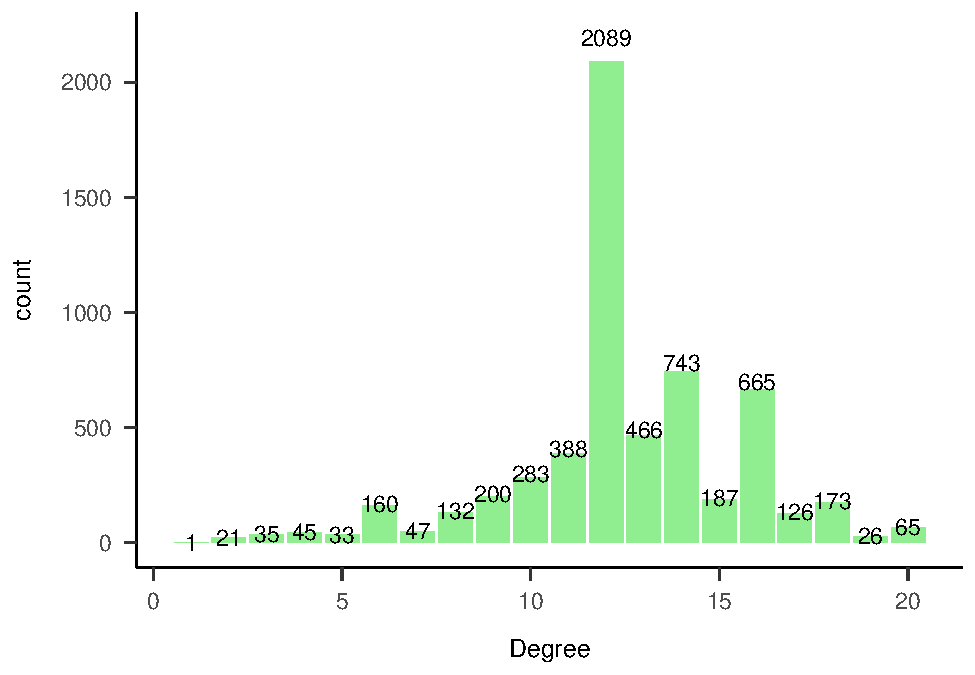
\includegraphics[keepaspectratio]{tables_files/figure-latex/unnamed-chunk-2-1.pdf}}
\caption{\label{fig:unnamed-chunk-2}a}
\end{figure}

\begin{figure}
\centering
\pandocbounded{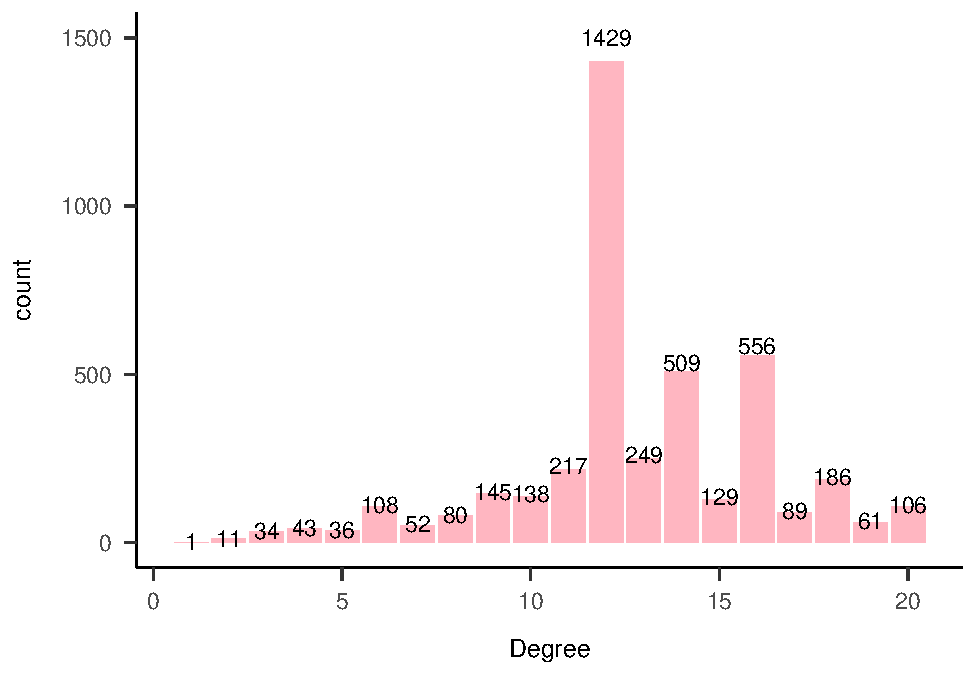
\includegraphics[keepaspectratio]{tables_files/figure-latex/unnamed-chunk-3-1.pdf}}
\caption{\label{fig:unnamed-chunk-3}row}
\end{figure}

• What were the results? • Provide descriptive statistics for key variables as well as results of data analysis • Data summaries are ok -- i.e.~tables \& charts

\begin{verbatim}
## # A tibble: 4 x 4
##   KEY_RACE_ETHNICITY_1997     n mom_missing_pct dad_missing_pct
##                     <int> <int>           <dbl>           <dbl>
## 1                       1  1808           14.7             59.9
## 2                       2  1391           12.4             40.2
## 3                       3    62           27.4             43.5
## 4                       4  3342            7.90            22.6
\end{verbatim}

\pandocbounded{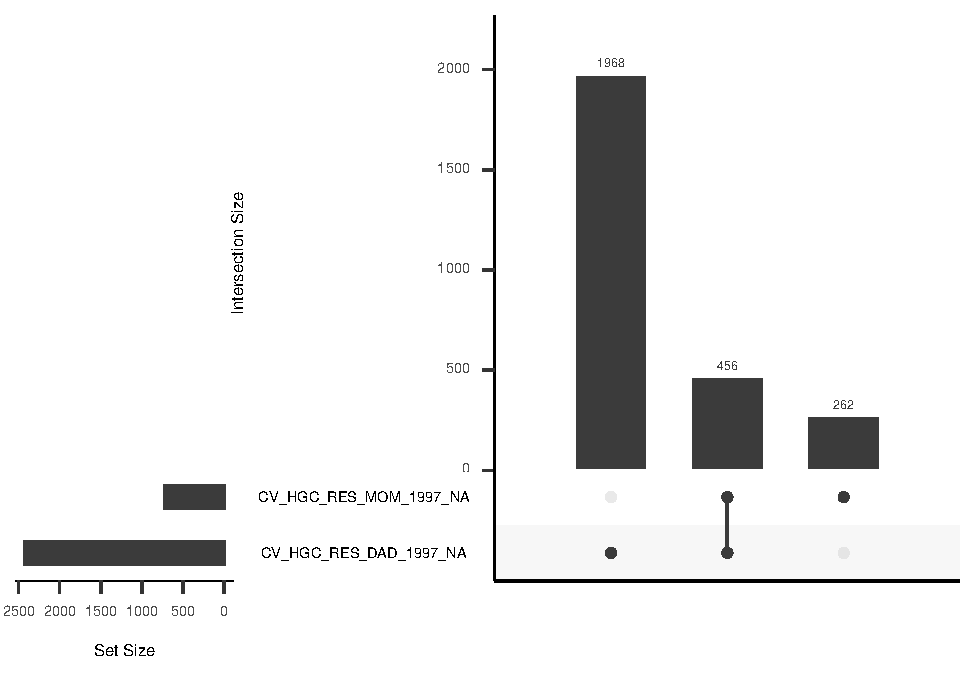
\includegraphics[keepaspectratio]{tables_files/figure-latex/unnamed-chunk-4-1.pdf}}

\begin{verbatim}
## # A tibble: 1 x 4
##   statistic    df p.value missing.patterns
##       <dbl> <dbl>   <dbl>            <int>
## 1      364.     5       0                4
\end{verbatim}

\begin{verbatim}
## Call:
## TestMCARNormality(data = mcar_data)
## 
## Number of Patterns:  4 
## 
## Total number of cases used in the analysis:  6603 
## 
##  Pattern(s) used:
##           CV_HIGHEST_DEGREE_EVER_EDT_2017   CV_HGC_RES_MOM_1997
## group.1                                 1                     1
## group.2                                 1                     1
## group.3                                 1                    NA
## group.4                                 1                    NA
##           CV_HGC_RES_DAD_1997   Number of cases
## group.1                     1              3917
## group.2                    NA              1968
## group.3                    NA               456
## group.4                     1               262
## 
## 
##     Test of normality and Homoscedasticity:
##   -------------------------------------------
## 
## Hawkins Test:
## 
##     P-value for the Hawkins test of normality and homoscedasticity:  3.397327e-131 
## 
##     Either the test of multivariate normality or homoscedasticity (or both) is rejected.
##     Provided that normality can be assumed, the hypothesis of MCAR is 
##     rejected at 0.05 significance level. 
## 
## Non-Parametric Test:
## 
##     P-value for the non-parametric test of homoscedasticity:  1.571686e-19 
## 
##     Hypothesis of MCAR is rejected at  0.05 significance level.
##     The multivariate normality test is inconclusive.
\end{verbatim}

\begin{verbatim}
## 
##  iter imp variable
##   1   1  CV_HGC_RES_MOM_1997  CV_HGC_RES_DAD_1997
##   1   2  CV_HGC_RES_MOM_1997  CV_HGC_RES_DAD_1997
##   1   3  CV_HGC_RES_MOM_1997  CV_HGC_RES_DAD_1997
##   1   4  CV_HGC_RES_MOM_1997  CV_HGC_RES_DAD_1997
##   1   5  CV_HGC_RES_MOM_1997  CV_HGC_RES_DAD_1997
##   2   1  CV_HGC_RES_MOM_1997  CV_HGC_RES_DAD_1997
##   2   2  CV_HGC_RES_MOM_1997  CV_HGC_RES_DAD_1997
##   2   3  CV_HGC_RES_MOM_1997  CV_HGC_RES_DAD_1997
##   2   4  CV_HGC_RES_MOM_1997  CV_HGC_RES_DAD_1997
##   2   5  CV_HGC_RES_MOM_1997  CV_HGC_RES_DAD_1997
##   3   1  CV_HGC_RES_MOM_1997  CV_HGC_RES_DAD_1997
##   3   2  CV_HGC_RES_MOM_1997  CV_HGC_RES_DAD_1997
##   3   3  CV_HGC_RES_MOM_1997  CV_HGC_RES_DAD_1997
##   3   4  CV_HGC_RES_MOM_1997  CV_HGC_RES_DAD_1997
##   3   5  CV_HGC_RES_MOM_1997  CV_HGC_RES_DAD_1997
##   4   1  CV_HGC_RES_MOM_1997  CV_HGC_RES_DAD_1997
##   4   2  CV_HGC_RES_MOM_1997  CV_HGC_RES_DAD_1997
##   4   3  CV_HGC_RES_MOM_1997  CV_HGC_RES_DAD_1997
##   4   4  CV_HGC_RES_MOM_1997  CV_HGC_RES_DAD_1997
##   4   5  CV_HGC_RES_MOM_1997  CV_HGC_RES_DAD_1997
##   5   1  CV_HGC_RES_MOM_1997  CV_HGC_RES_DAD_1997
##   5   2  CV_HGC_RES_MOM_1997  CV_HGC_RES_DAD_1997
##   5   3  CV_HGC_RES_MOM_1997  CV_HGC_RES_DAD_1997
##   5   4  CV_HGC_RES_MOM_1997  CV_HGC_RES_DAD_1997
##   5   5  CV_HGC_RES_MOM_1997  CV_HGC_RES_DAD_1997
\end{verbatim}

\begin{verbatim}
##                      term  estimate  std.error statistic        df
## 1     CV_HGC_RES_MOM_1997 0.1129312 0.01120928 10.074796  147.9423
## 2 KEY_RACE_ETHNICITY_1997 0.1602952 0.01864827  8.595714  520.2339
## 3     CV_HGC_RES_DAD_1997 0.1438466 0.01007570 14.276589  146.9429
## 4                None|GED 0.9226579 0.11554605  7.985196 1258.2747
## 5                  GED|HS 2.1366787 0.11384089 18.768992  860.9647
## 6                   HS|AA 4.1726090 0.12280189 33.978378  696.8323
## 7                   AA|BA 4.6396842 0.12554164 36.957332  676.3646
## 8                   BA|MA 6.2373973 0.13624590 45.780441  727.2976
## 9                  MA|PhD 8.8384867 0.19316239 45.756767 1944.3151
##         p.value
## 1  1.677571e-18
## 2  9.731862e-17
## 3  1.482680e-29
## 4  3.141361e-15
## 5  3.770730e-66
## 6 5.338332e-150
## 7 1.877171e-164
## 8 2.180449e-216
## 9 6.882897e-311
\end{verbatim}

\pandocbounded{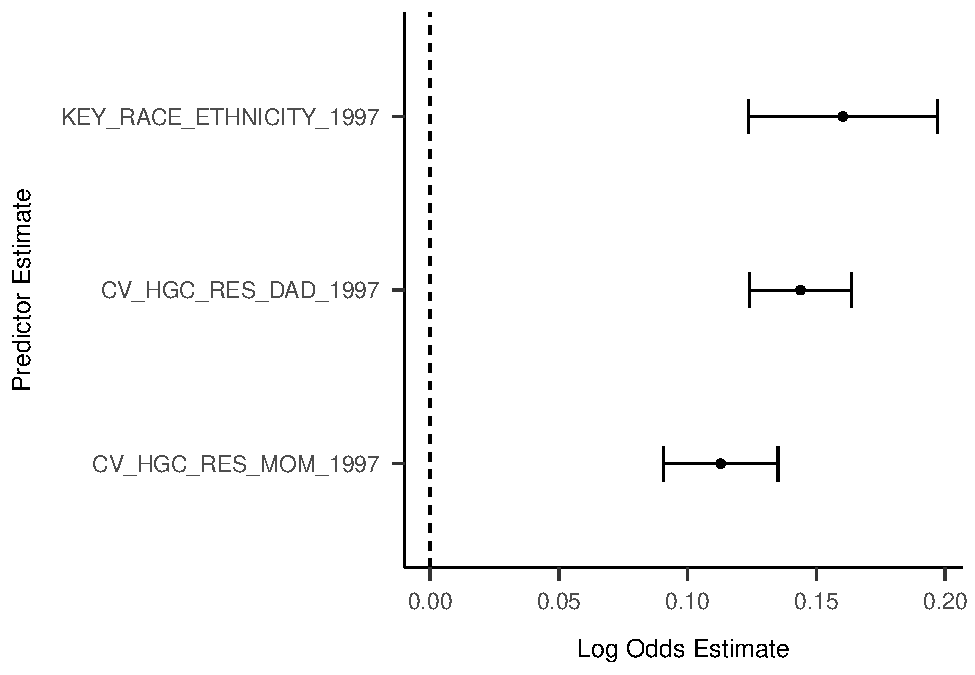
\includegraphics[keepaspectratio]{tables_files/figure-latex/unnamed-chunk-4-2.pdf}} \pandocbounded{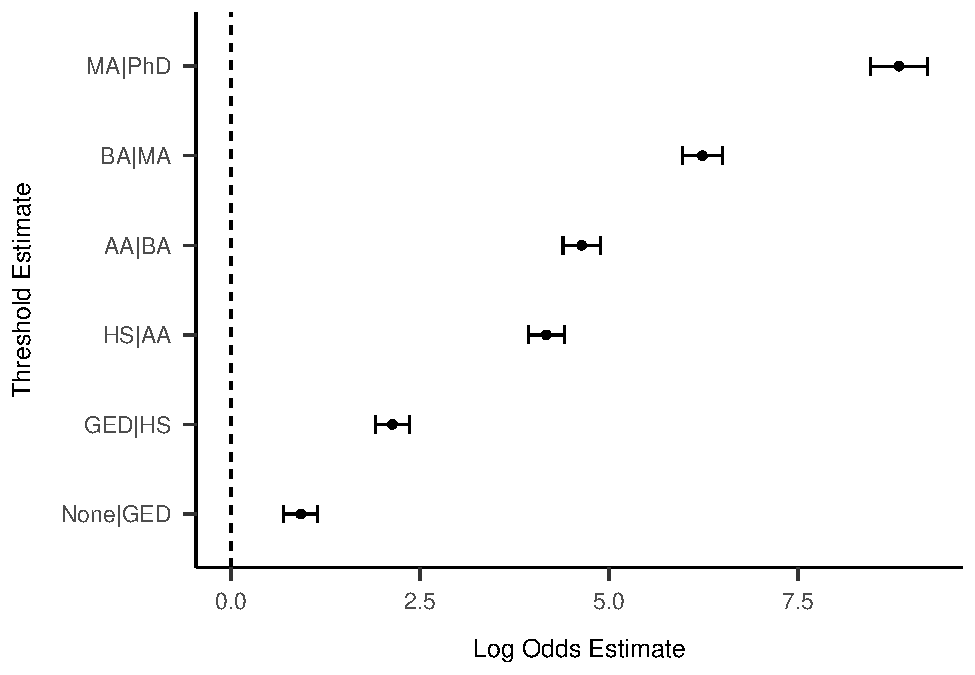
\includegraphics[keepaspectratio]{tables_files/figure-latex/unnamed-chunk-4-3.pdf}}

\begin{verbatim}
## 
## Call:
## svyglm(formula = degree_num ~ CV_HGC_RES_MOM_1997 + KEY_RACE_ETHNICITY_1997 + 
##     CV_HGC_RES_DAD_1997, design = svy_design)
## 
## Survey design:
## svydesign(ids = ~1, weights = ~SAMPLING_WEIGHT_CC_2017, data = completed_data)
## 
## Coefficients:
##                         Estimate Std. Error t value Pr(>|t|)    
## (Intercept)             0.591379   0.082831   7.140 1.04e-12 ***
## CV_HGC_RES_MOM_1997     0.088172   0.008338  10.574  < 2e-16 ***
## KEY_RACE_ETHNICITY_1997 0.094713   0.013034   7.267 4.11e-13 ***
## CV_HGC_RES_DAD_1997     0.121326   0.006960  17.432  < 2e-16 ***
## ---
## Signif. codes:  0 '***' 0.001 '**' 0.01 '*' 0.05 '.' 0.1 ' ' 1
## 
## (Dispersion parameter for gaussian family taken to be 1.623647)
## 
## Number of Fisher Scoring iterations: 2
\end{verbatim}

\begin{verbatim}
##    KEY_RACE_ETHNICITY_1997 CV_HGC_RES_MOM_1997      fit         se    lower
## 1                      1.0                 1.0 2.356420 0.10055290 2.159304
## 2                      1.8                 1.0 2.432191 0.09983960 2.236473
## 3                      2.5                 1.0 2.498491 0.10010621 2.302250
## 4                      3.2                 1.0 2.564790 0.10119809 2.366409
## 5                      4.0                 1.0 2.640561 0.10342204 2.437820
## 6                      1.0                 5.8 2.779645 0.06329052 2.655575
## 7                      1.8                 5.8 2.855416 0.06132908 2.735191
## 8                      2.5                 5.8 2.921715 0.06103899 2.802059
## 9                      3.2                 5.8 2.988015 0.06210275 2.866273
## 10                     4.0                 5.8 3.063785 0.06488700 2.936586
## 11                     1.0                10.0 3.149967 0.03594049 3.079512
## 12                     1.8                10.0 3.225737 0.03095931 3.165047
## 13                     2.5                10.0 3.292037 0.02907362 3.235043
## 14                     3.2                10.0 3.358336 0.02997604 3.299574
## 15                     4.0                10.0 3.434107 0.03410759 3.367245
## 16                     1.0                15.0 3.590826 0.03548223 3.521269
## 17                     1.8                15.0 3.666597 0.02863611 3.610460
## 18                     2.5                15.0 3.732896 0.02478542 3.684309
## 19                     3.2                15.0 3.799195 0.02398120 3.752184
## 20                     4.0                15.0 3.874966 0.02709504 3.821851
## 21                     1.0                20.0 4.031685 0.06857514 3.897255
## 22                     1.8                20.0 4.107456 0.06448151 3.981051
## 23                     2.5                20.0 4.173755 0.06212608 4.051968
## 24                     3.2                20.0 4.240054 0.06105673 4.120364
## 25                     4.0                20.0 4.315825 0.06149183 4.195281
##       upper
## 1  2.553537
## 2  2.627909
## 3  2.694731
## 4  2.763171
## 5  2.843301
## 6  2.903715
## 7  2.975641
## 8  3.041371
## 9  3.109756
## 10 3.190985
## 11 3.220422
## 12 3.286428
## 13 3.349031
## 14 3.417099
## 15 3.500969
## 16 3.660382
## 17 3.722733
## 18 3.781483
## 19 3.846206
## 20 3.928081
## 21 4.166114
## 22 4.233860
## 23 4.295542
## 24 4.359745
## 25 4.436369
\end{verbatim}

\section{Analysis (1.5-2.5 pg)}\label{analysis-1.5-2.5-pg}

• What patterns are there in the responses? Discuss how these might shed light on your research question. On your hypothesis? • Is the data strong enough to make a conclusion for your hypothesis? How do you know?

\section{Discussion (1.5-2.5pg)}\label{discussion-1.5-2.5pg}

\newpage

\section{References}\label{references}

\phantomsection\label{refs}
\begin{CSLReferences}{1}{0}
\bibitem[\citeproctext]{ref-vanbuuren2018}
Buuren, S. van. (2018). \emph{Https://stefvanbuuren.name/fimd/sec-pmm.html} (2nd ed.). Chapman; Hall/CRC. Retrieved from \url{https://stefvanbuuren.name/fimd/sec-pmm.html}

\bibitem[\citeproctext]{ref-jamshidian2010}
Jamshidian, M., \& Jalal, S. (2010). Tests of homoscedasticity, normality, and missing completely at random for incomplete multivariate data. \emph{Psychometrika}, \emph{75}(4), 649--674. \url{https://doi.org/10.1007/s11336-010-9175-3}

\end{CSLReferences}

\newpage

\appendix


R00001.00 {[}PUBID{]} Survey Year: 1997
PRIMARY VARIABLE

\begin{verbatim}
         PUBID, YOUTH CASE IDENTIFICATION CODE
\end{verbatim}

COMMENT: YOUTH CASE IDENTIFICATION CODE

\begin{verbatim}
   0           0
 998           1 TO 999
 999        1000 TO 1999
 997        2000 TO 2999
 996        3000 TO 3999
 998        4000 TO 4999
 996        5000 TO 5999
 994        6000 TO 6999
 994        7000 TO 7999
 989        8000 TO 8999
  23        9000 TO 9999
\end{verbatim}

\begin{longtable}[]{@{}
  >{\centering\arraybackslash}p{(\linewidth - 0\tabcolsep) * \real{0.1111}}@{}}
\toprule\noalign{}
\begin{minipage}[b]{\linewidth}\centering
8984
\end{minipage} \\
\midrule\noalign{}
\endhead
\bottomrule\noalign{}
\endlastfoot
8984 \\
fusal(-1) 0
n't Know(-2) 0
TAL =========\textgreater{} 8984 VALID SKIP(-4) 0 NON-INTERVIEW(-5) 0 \\
n: 1 Max: 2 Mean: 1.49 \\
ad In: R00001.00{[}Default{]}
fault Next Question: R05364.00 \\
5364.01 {[}KEY!BDATE\_M{]} Survey Year: 1997
PRIMARY VARIABLE \\
KEY!BDATE, RS BIRTHDATE MONTH/YEAR (SYMBOL) \\
MMENT: Birthdate of Youth \\
816 1: January
693 2: February
760 3: March
659 4: April
689 5: May
720 6: June
762 7: July
782 8: August
839 9: September
765 10: October
763 11: November
736 12: December \\
\end{longtable}

\begin{verbatim}
8984
\end{verbatim}

Refusal(-1) 0
Don't Know(-2) 0
TOTAL =========\textgreater{} 8984 VALID SKIP(-4) 0 NON-INTERVIEW(-5) 0

Min: 1 Max: 12 Mean: 6.56

Earliest (NonMissing): JANUARY/1980
Latest (NonMissing): DECEMBER/1984

Lead In: None.
Default Next Question: R05364.02
--------------------------------------------------------------------------------
R05364.02 {[}KEY!BDATE\_Y{]} Survey Year: 1997
PRIMARY VARIABLE

\begin{verbatim}
         KEY!BDATE, RS BIRTHDATE MONTH/YEAR (SYMBOL)
\end{verbatim}

COMMENT: Birthdate of Youth

Refusal(-1) 0
Don't Know(-2) 0
TOTAL =========\textgreater{} 8984 VALID SKIP(-4) 0 NON-INTERVIEW(-5) 0

Min: 1980 Max: 1984 Mean: 1982.01

Earliest (NonMissing): JANUARY/1980
Latest (NonMissing): DECEMBER/1984

Lead In: R05364.01{[}Default{]}
Default Next Question: R05366.00
--------------------------------------------------------------------------------
R12358.00 {[}CV\_SAMPLE\_TYPE{]} Survey Year: 1997
PRIMARY VARIABLE

\begin{verbatim}
         SAMPLE TYPE.  CROSS-SECTIONAL OR OVERSAMPLE
\end{verbatim}

Sample type: Is the respondent a member of the cross-sectional sample or the
oversample?

\begin{verbatim}
6748       1 Cross-sectional
2236       0 Oversample
\end{verbatim}

\begin{longtable}[]{@{}
  >{\centering\arraybackslash}p{(\linewidth - 0\tabcolsep) * \real{1.0000}}@{}}
\toprule\noalign{}
\begin{minipage}[b]{\linewidth}\centering
8984
\end{minipage} \\
\midrule\noalign{}
\endhead
\bottomrule\noalign{}
\endlastfoot
R12361.01 {[}SAMPLING\_WEIGHT\_CC{]} Survey Year: 1997
PRIMARY VARIABLE \\
ROUND 1 SAMPLING WEIGHT CUMULATIVE CASES METHOD \\
Sampling Weight: Cumulative Cases Method 0 thru 9999999 (2 implied decimal
places) \\
NOTE: 0 THRU 9999999 (2 IMPLIED DECIMAL PLACES) \\
0 0
0 30000 TO 59999: 300.00-599.99
1445 60000 TO 99999: 600.00-999.99
1883 100000 TO 149999: 1000.00-1499.99
214 150000 TO 199999: 1500.00-1999.99
514 200000 TO 249999: 2000.00-2499.99
3354 250000 TO 299999: 2500.00-2999.99
1442 300000 TO 349999: 3000.00-3499.99
97 350000 TO 399999: 3500.00-3999.99
22 400000 TO 449999: 4000.00-4499.99
8 450000 TO 499999: 4500.00-4999.99
4 500000 TO 549999: 5000.00-5499.99
0 550000 TO 599999: 5500.00-5999.99
0 600000 TO 649999: 6000.00-6499.99
0 650000 TO 699999: 6500.00-6999.99
0 700000 TO 749999: 7000.00-7499.99
0 750000 TO 799999: 7500.00-7999.99
0 800000 TO 849999: 8000.00-8499.99
1 850000 TO 9999999: 8500.00+ \\
\end{longtable}

\begin{verbatim}
8984
\end{verbatim}

Refusal(-1) 0
Don't Know(-2) 0
TOTAL =========\textgreater{} 8984 VALID SKIP(-4) 0 NON-INTERVIEW(-5) 0

Min: 76071 Max: 1576182 Mean: 215699.61

Lead In: R12361.00{[}Default{]}
Default Next Question: R12362.01
--------------------------------------------------------------------------------
R13026.00 {[}CV\_HGC\_RES\_DAD{]} Survey Year: 1997
PRIMARY VARIABLE

\begin{verbatim}
         RESIDENTIAL FATHERS HIGHEST GRADE COMPLETED
\end{verbatim}

Highest grade completed by respondent's residential father (includes both
biological and non-biological fathers).

\begin{verbatim}
   0       0 NONE
   1       1 1ST GRADE
  12       2 2ND GRADE
  51       3 3RD GRADE
  56       4 4TH GRADE
  51       5 5TH GRADE
 150       6 6TH GRADE
  69       7 7TH GRADE
 117       8 8TH GRADE
 186       9 9TH GRADE
 195      10 10TH GRADE
 277      11 11TH GRADE
1917      12 12TH GRADE
 345      13 1ST YEAR COLLEGE
 720      14 2ND YEAR COLLEGE
 164      15 3RD YEAR COLLEGE
 780      16 4TH YEAR COLLEGE
 119      17 5TH YEAR COLLEGE
 255      18 6TH YEAR COLLEGE
  86      19 7TH YEAR COLLEGE
 153      20 8TH YEAR COLLEGE OR MORE
   3      95 UNGRADED
\end{verbatim}

\begin{longtable}[]{@{}
  >{\centering\arraybackslash}p{(\linewidth - 0\tabcolsep) * \real{1.0000}}@{}}
\toprule\noalign{}
\begin{minipage}[b]{\linewidth}\centering
5707
\end{minipage} \\
\midrule\noalign{}
\endhead
\bottomrule\noalign{}
\endlastfoot
R13027.00 {[}CV\_HGC\_RES\_MOM{]} Survey Year: 1997
PRIMARY VARIABLE \\
RESIDENTIAL MOTHERS HIGHEST GRADE COMPLETED \\
Highest grade completed by respondent's residential mother (includes both
biological and non-biological mothers). \\
0 0 NONE
3 1 1ST GRADE
28 2 2ND GRADE
51 3 3RD GRADE
54 4 4TH GRADE
54 5 5TH GRADE
221 6 6TH GRADE
67 7 7TH GRADE
183 8 8TH GRADE
260 9 9TH GRADE
373 10 10TH GRADE
517 11 11TH GRADE
2870 12 12TH GRADE
639 13 1ST YEAR COLLEGE
996 14 2ND YEAR COLLEGE
251 15 3RD YEAR COLLEGE
902 16 4TH YEAR COLLEGE
163 17 5TH YEAR COLLEGE
246 18 6TH YEAR COLLEGE
38 19 7TH YEAR COLLEGE
89 20 8TH YEAR COLLEGE OR MORE
5 95 UNGRADED \\
\end{longtable}

\begin{verbatim}
8010
\end{verbatim}

Refusal(-1) 0
Don't Know(-2) 0
Invalid Skip(-3) 316
TOTAL =========\textgreater{} 8326 VALID SKIP(-4) 658 NON-INTERVIEW(-5) 0

Min: 1 Max: 95 Mean: 12.58

Lead In: R13026.00{[}Default{]}
Default Next Question: R12045.00
--------------------------------------------------------------------------------
R14826.00 {[}KEY!RACE\_ETHNICITY{]} Survey Year: 1997
PRIMARY VARIABLE

\begin{verbatim}
         KEY!RACE_ETHNICITY, COMBINED RACE AND ETHNICITY (SYMBOL)
\end{verbatim}

COMMENT: Combined race - ethnicity variable

\begin{verbatim}
2335       1 Black
1901       2 Hispanic
  83       3 Mixed Race (Non-Hispanic)
4665       4 Non-Black / Non-Hispanic
\end{verbatim}

\begin{longtable}[]{@{}
  >{\centering\arraybackslash}p{(\linewidth - 0\tabcolsep) * \real{1.0000}}@{}}
\toprule\noalign{}
\begin{minipage}[b]{\linewidth}\centering
8984
\end{minipage} \\
\midrule\noalign{}
\endhead
\bottomrule\noalign{}
\endlastfoot
U18460.00 {[}CV\_HIGHEST\_DEGREE\_EVER\_EDT{]} Survey Year: 2017
PRIMARY VARIABLE \\
HIGHEST DEGREE RECEIVED \\
The highest degree received as of the survey date. \\
514 0 None
862 1 GED
2692 2 High school diploma (Regular 12 year program)
598 3 Associate/Junior college (AA)
1352 4 Bachelor's degree (BA, BS)
540 5 Master's degree (MA, MS)
51 6 PhD
98 7 Professional degree (DDS, JD, MD) \\
\end{longtable}

\begin{verbatim}
6707
\end{verbatim}

Refusal(-1) 0
Don't Know(-2) 0
Invalid Skip(-3) 27
TOTAL =========\textgreater{} 6734 VALID SKIP(-4) 0 NON-INTERVIEW(-5) 2250

Min: 0 Max: 7 Mean: 2.56

Lead In: U18459.00{[}Default{]}
Default Next Question: U18461.00
--------------------------------------------------------------------------------
U18554.00 {[}SAMPLING\_WEIGHT\_CC{]} Survey Year: 2017
PRIMARY VARIABLE

\begin{verbatim}
         ROUND 18 SAMPLING WEIGHT CUMULATIVE CASES METHOD
\end{verbatim}

Sampling Weight: Cumulative Cases Method 0 thru 9999999 (2 implied decimal
places)

NOTE: 0 THRU 9999999 (2 IMPLIED DECIMAL PLACES)

\begin{verbatim}
2250           0
   0       30000 TO 59999: 300.00-599.99
  83       60000 TO 99999: 600.00-999.99
1882      100000 TO 149999: 1000.00-1499.99
 588      150000 TO 199999: 1500.00-1999.99
 157      200000 TO 249999: 2000.00-2499.99
 272      250000 TO 299999: 2500.00-2999.99
 346      300000 TO 349999: 3000.00-3499.99
2019      350000 TO 399999: 3500.00-3999.99
 938      400000 TO 449999: 4000.00-4499.99
 384      450000 TO 499999: 4500.00-4999.99
  30      500000 TO 549999: 5000.00-5499.99
  20      550000 TO 599999: 5500.00-5999.99
  10      600000 TO 649999: 6000.00-6499.99
   2      650000 TO 699999: 6500.00-6999.99
   1      700000 TO 749999: 7000.00-7499.99
   1      750000 TO 799999: 7500.00-7999.99
   0      800000 TO 849999: 8000.00-8499.99
   1      850000 TO 9999999: 8500.00+
\end{verbatim}

\begin{center}\rule{0.5\linewidth}{0.5pt}\end{center}

\begin{verbatim}
8984
\end{verbatim}

Refusal(-1) 0
Don't Know(-2) 0
TOTAL =========\textgreater{} 8984 VALID SKIP(-4) 0 NON-INTERVIEW(-5) 0

Min: 0 Max: 2007281 Mean: 215699.61

Lead In: U18553.00{[}Default{]}
Default Next Question: U18555.00


\end{document}
